\begin{frame}{Scan Theory}
	\begin{itemize}
		\item names: prefix sum, cumulative sum or scan
		\item inclusive and exclusive version
		\item further specialization: segmented scan
	\end{itemize}
\end{frame} 
\begin{frame}{Inclusive Scan}
	\begin{figure}
		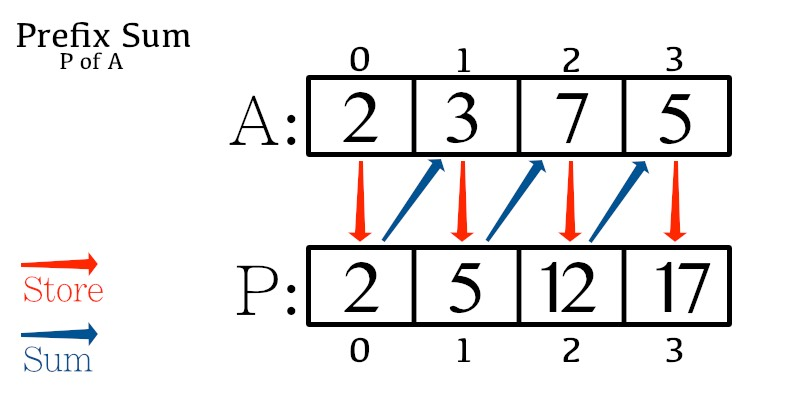
\includegraphics[width=80mm]{wiki/prefix-sum.jpg}
		\caption{{calculation of an inclusive prefix sum\\ \tiny https://williamrjribeiro.com/?p=132}}
	\end{figure}
\end{frame}
\begin{frame}{inclusive vs. exclusive scan}
	\begin{figure}
		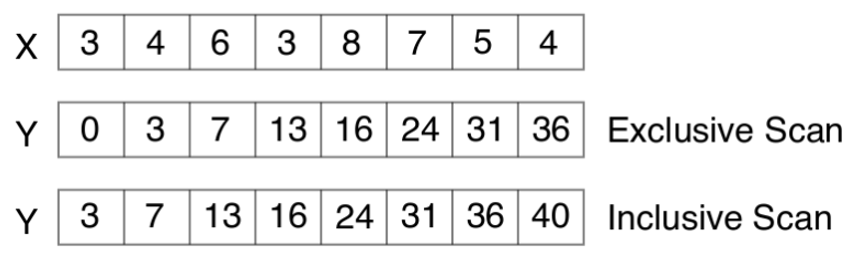
\includegraphics[width=80mm]{wiki/scans.png}
		\caption{{\tiny https://livebook.manning.com/book/parallel-and-high-performance-computing/chapter-5/v-11/}}
	\end{figure}
\end{frame}
\begin{frame}{segmented variant}
	\begin{figure}
		%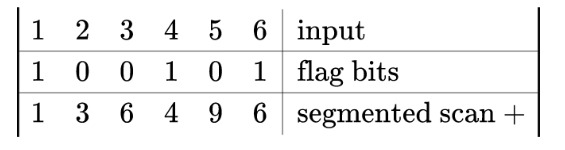
\includegraphics[width=80mm]{wiki/SegmentedScan.png}
		\caption{{segmented scan \\ \tiny https://en.wikipedia.org/wiki/Segmented\_scan}}
	\end{figure}
\end{frame}

